\documentclass[serif]{beamer}
\usepackage[T1]{fontenc}
\usepackage{concmath}
\usepackage{amsmath}
\usepackage{amsfonts}
\usepackage{amssymb}
\usepackage{amsthm}
\newcommand{\ZZ}{\mathbb{Z}}
\newcommand{\HH}{\mathbb{H}}
\newcommand{\CC}{\mathbb{C}}
\title{Continued Fractions and Hyperbolic Geometry}
\author{Math Club Week 9}
\date{May 24, 2021}
\begin{document}

\frame{\titlepage}

\begin{frame}{Today I will...}
    \begin{itemize}
        \item ...discuss the basics of continued fractions: what are they, how to compute them, why we care.
        \item ...review the upper half plane model in hyperbolic geometry, and introduce the Farey tesselation in the upper half plane.
        \item ...unveil a stunning link between continued fraction expansions and hyperbolic geometry!
        \item ...or possibly just the first one depending on time.
    \end{itemize}
\end{frame}

\begin{frame}{A quickie intro to continued fractions}
    \begin{itemize}
        \item At the most basic level, a continued fraction is just a new way to represent numbers. 
        \item Useful in quantum mechanics, statistics, and especially number theory.
    \end{itemize}
\end{frame}

\begin{frame}{What is a continued fraction?}
    \begin{definition}
    A \emph{continued fraction} is an expression of the form 
    \[a_1+\cfrac{1}{a_2+\cfrac{1}{a_3+\cfrac{1}{\dots}}}\ \ \ \ \text{ or }\ \ \ \ a_1+\cfrac{1}{a_2+\cfrac{1}{a_3+\cfrac{1}{\cfrac{\ddots}{a_{n-1}+\frac{1}{a_n}}}}}
    \] We will be working with \emph{simple} continued fractions, that is, fractions where all of the numbers $a_1,a_2,a_3,\dots$ are \emph{positive integers}.
    \end{definition}
\end{frame}

\begin{frame}{Examples of continued fractions}
    A continued fraction can be either \emph{finite}:
    \[3 + \cfrac{1}{2 + \cfrac{1}{4+\cfrac{1}{5}}}
    \] or 
    \emph{infinite}:
    \[1 +\cfrac{1}{1+\cfrac{1}{1+\cfrac{1}{1+\cdots}}}
    \]
    But it is important to see that continued fractions \emph{are just numbers represented in a different way}.
\end{frame}

\begin{frame}{A fundamental theorem}
    \begin{theorem}
    Every real number $x$, rational or irrational, can be represented uniquely as a continued fraction:
    \[x = a_1 + \cfrac{1}{a_2+\cfrac{1}{a_3+\cfrac{1}{\dots}}}
    \] If $x$ is rational, this continued fraction will be finite. Otherwise, it will be infinite.
    \end{theorem}
\end{frame}

\begin{frame}{An important fact}
    \begin{theorem}
    Let $x$ be a real number. Then $x$ can be uniquely written as \[x=n+\theta\] where $n\in \ZZ$ and $0\leqslant \theta < 1$. We call $n$ the ``integer part'' of $x$, and we call $\theta$ the ``fractional part'' of $x$.
    \end{theorem}
\end{frame}

\begin{frame}{Compute!}
    Let's compute the continued fraction expansion of a rational number.
\end{frame}

\begin{frame}{Compute!}
    Let's compute the continued fraction expansion of an irrational number: $\sqrt{2}$. It may help to have a calculator handy!
\end{frame}

\begin{frame}{Problem 1}
    Compute the continued fraction expansion of \emph{the golden mean}: $\frac{1+\sqrt{5}}{2}$.
\end{frame}

\begin{frame}{Notation change}
    NOTATION: It is too cumbersome to write \[a_1+\cfrac{1}{a_2+\cfrac{1}{a_3+\cdots}}\]
    so I will simply write $[a_1;a_2,a_3,\dots]$, with the understanding that the above is what I really mean. If the expansion is finite, I will just write $[a_1;a_2,a_3,\dots,a_n]$.
\end{frame}

\begin{frame}{Some fun facts about continued fractions}
    \begin{itemize}
        \item The real number $x$ has a periodic continued fraction expansion if and only if it is a quadratic irrational.
        \item Weirdly, the continued fraction for $e$ has a pretty clear pattern:
        \[e = [2;1,2,1,1,4,1,1,6,1,1,8,\dots]\]
        \item The expansion for $\pi$ is not nearly as simple:
        \[\pi = [3;7,15,1,292, 1,1,1,2,1,3,1,\dots]\]
    \end{itemize}
\end{frame}

\begin{frame}{Open Problem!}
    Is there a pattern in the continued fraction expansion of $\sqrt[3]{2}$? Here are the first few terms:
    \begin{multline*}
        [1;3,1,5,1,1,4,1,1,8,1,14,1,10,2,1,4,12, 2,3,2,1,3,4,1,1, 
        \\2,14,3,12,1,15,3,1,4,
        534,1,1,5,1,1,\dots]
    \end{multline*}
\end{frame}

\begin{frame}{Problem 2}
    Find the irrational number having continued fraction expansion $[8;1,16,1,16,1,16,\dots]$.
    
\end{frame}


\begin{frame}{Experts only}
Let $p\equiv 1 \pmod{4}$ be a prime number, and choose an integer $u$ such that $u^2\equiv -1 \pmod{4}$. Suppose $u/p$ has continued fraction expansion $[a_0;a_1,\dots,a_n]$, and denote by $h_j/k_j$ its $j$-th convergent, for $j=0,1,\dots,n$. Prove that if $i$ is the greatest integer such that $k_i\leqslant \sqrt{p}$, then \[x=k_i,\ \ \ \ y=h_ip-uk_i\] defines an integer solution $(x,y)$ to the equation $x^2+y^2=p$.
\end{frame}

\begin{frame}{The ``real'' significance of continued fractions}
    Suppose $x$ is an irrational number with (simple) continued fraction expansion $x=[a_1;a_2,a_3,a_4,\dots]$. The \emph{convergents} are the rational numbers $[a_1]$, $[a_1;a_2]$, $[a_1;a_2,a_3]$, \dots, and they represent the \emph{best rational approximations to $x$ up to denominator}.
\end{frame}

\begin{frame}{Example: $\pi$}
    So $\pi=[3;7,15,1,292,1,1,1,2,1,3,1,\dots]$. Its convergents are 
    \begin{align*}
        [3] &= 3 \\
        [3;7] &= 3+\frac{1}{7}=\frac{22}{7} =3.142\dots \\
        [3;7,15] &= 3 + \frac{1}{7+\frac{1}{15}}=\frac{333}{106}=3.14150\dots \\
        [3;7,15,1] &= 3 + \frac{1}{7+\frac{1}{15+\frac{1}{1}}}=\frac{355}{113}=3.1415929\dots
    \end{align*}
\end{frame}

\begin{frame}{Upshot}
    By truncating the continued fraction expansion, we obtain a sequence of really good rational approximations to any irrational number we want. 
    
    The ``convergents'' are extremely easy to compute, which leads to innumerable applications (example: finding an explicit representation of a number $n$ as the sum of two squares $n=a^2+b^2$).
\end{frame}

\begin{frame}{References for Continued Fractions}
    \begin{itemize}
        \item Chapter $5$ of \emph{Elementary Number Theory: Primes, Congruences, and Secrets} by William Stein.
        \item Chapter $7$ of \emph{Introduction to the Theory of Numbers} by Niven and Zuckerman. 
        \item \emph{Continued Fractions} by Khinchin.
    \end{itemize}
\end{frame}

\begin{frame}{Recall: Hyperbolic Geometry}
    We now turn to the upper half plane $\HH=\{z\in \CC\ :\ \operatorname{Im}{z}>0\}$.
    
    Recall the \emph{geodesics} (just think of them as the analogues to ``lines'' in Euclidean geometry) are semicircles which connect two points on the real axis and vertical lines. 
\end{frame}

\begin{frame}{The Farey Tesselation}
    The \emph{Farey Tesselation} is a tiling of the upper half plane $\HH$: that is, a subdivision of $\HH$ into regions by geodesics.
    
    It is the fundamental link that allows us to view arithmetical questions concerning continued fractions through the lens of hyperbolic geometry.
\end{frame}

\begin{frame}{Constructing the Farey Tesselation}
    Construct the Farey tesselation as follows.
    \begin{itemize}
        \item For each integer $n\in \ZZ$, draw a vertical line from $n$ extending upward. 
        \item For each consecutive pair of integers $n$ and $n+1$, draw the semicircle in $\HH$ which connects $n$ and $n+1$.
        \item Now follow this rule: if $p/q$ and $r/s$ are two consecutive numbers which are joined by a semicircle, then join $p/q$ to $(p+r)/(q+s)$ by a semicircle and $(p+r)/(q+s)$ to $r/s$ by a semicircle.
        \item Recursively repeat step 3.
    \end{itemize}
\end{frame}

\begin{frame}{Let's Draw!}
    
\end{frame}

\begin{frame}{The Farey Tesselation}
    It looks like this by the time we're done.
    \begin{figure}
        \centering
        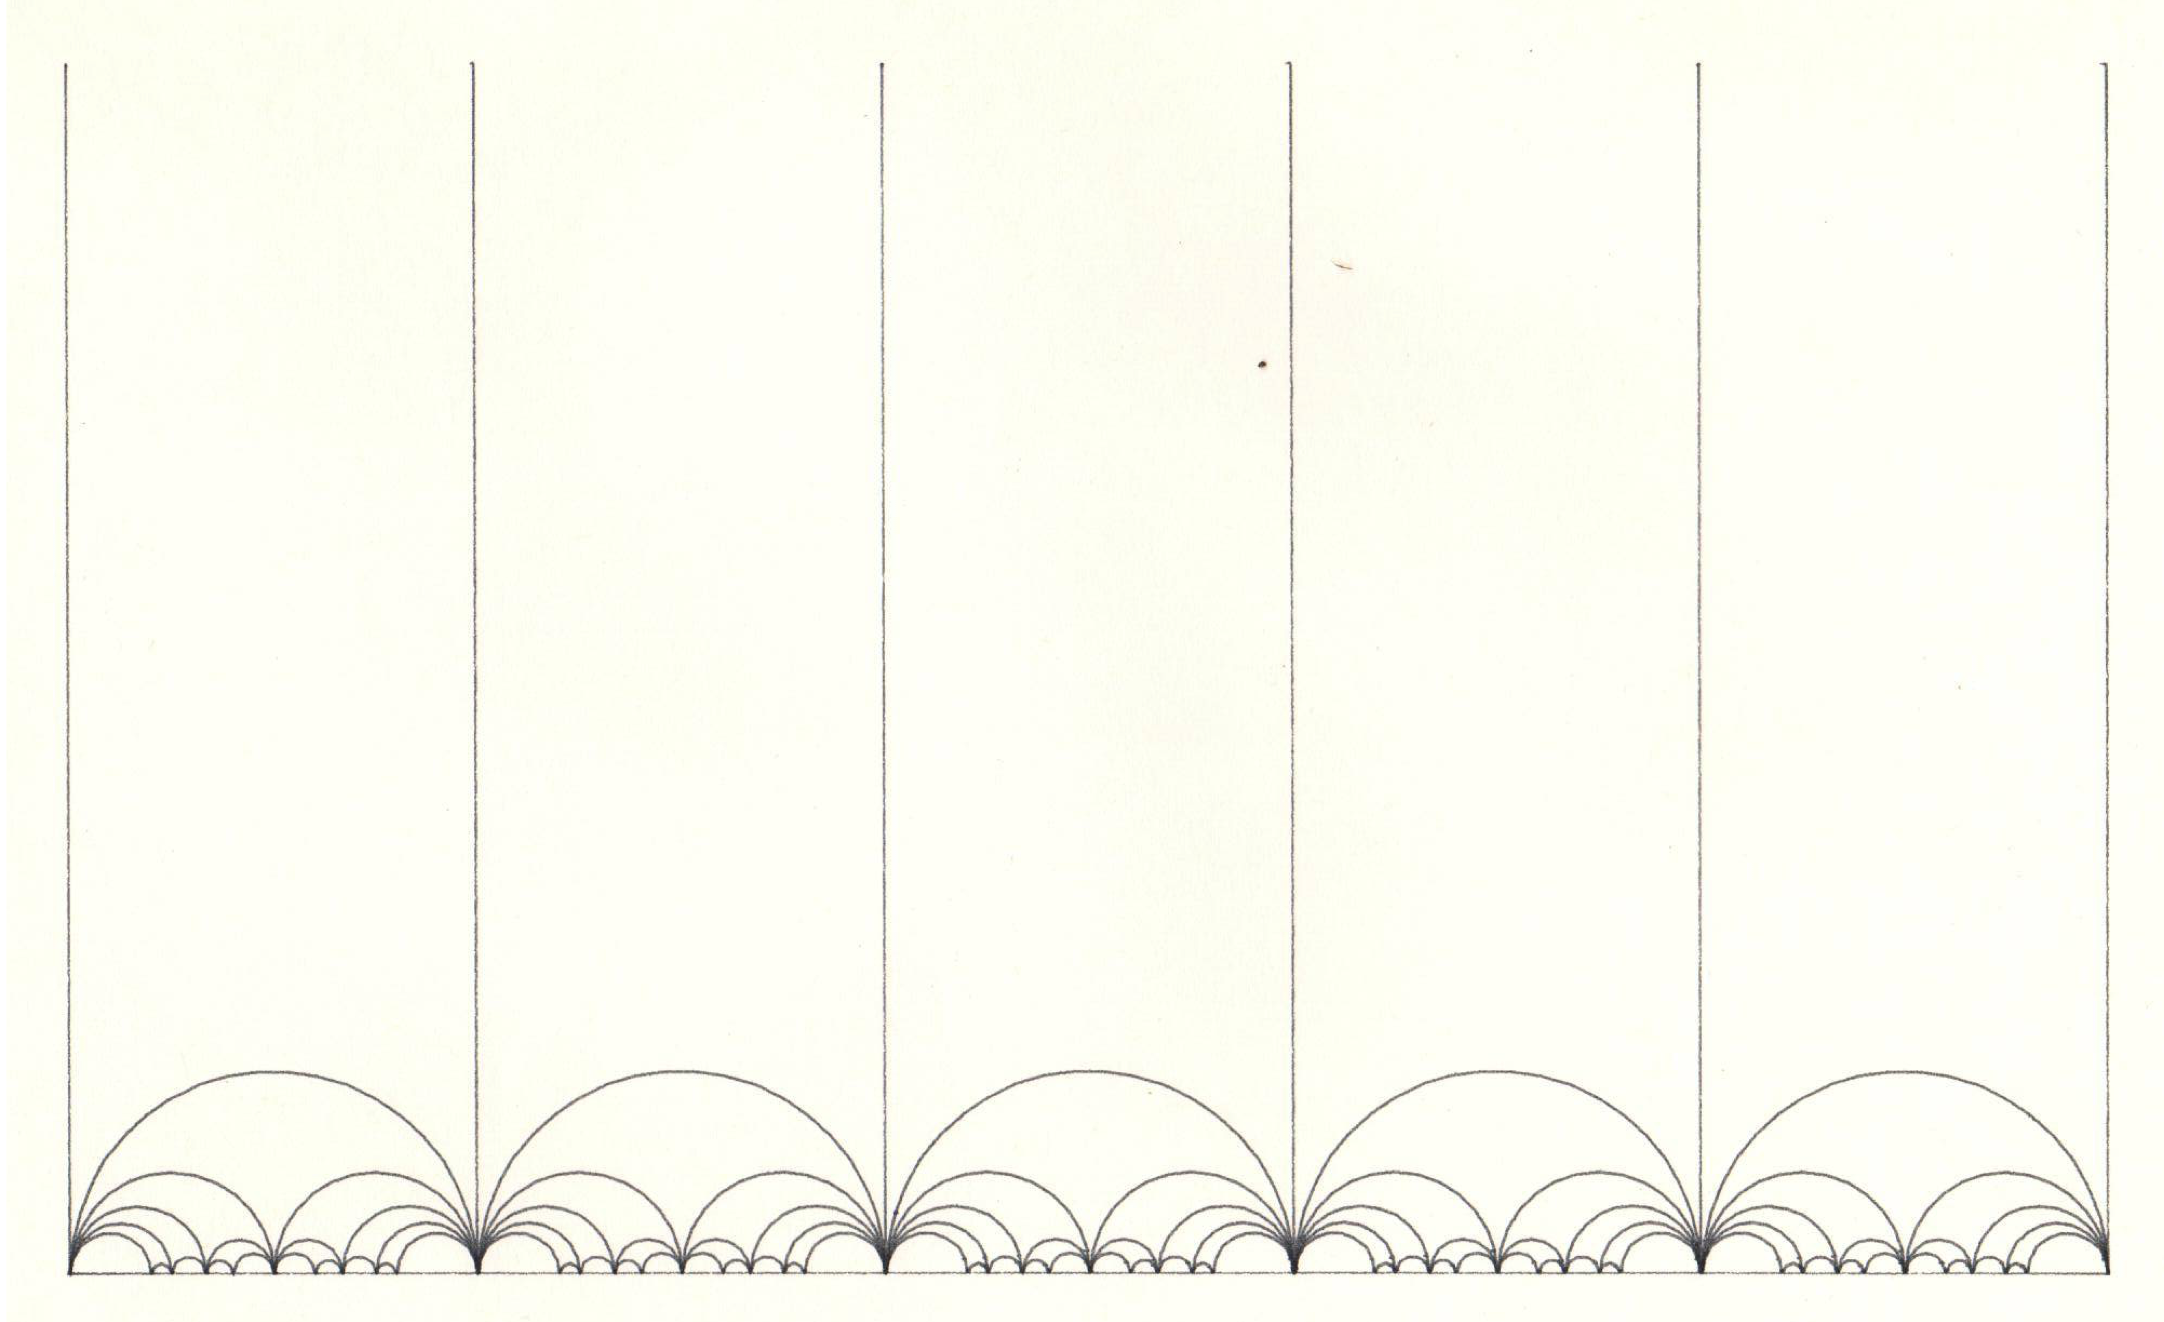
\includegraphics[scale=0.25]{pics/farey.png}
        \caption{The Farey Tesselation}
    \end{figure}
\end{frame}

\begin{frame}{The cutting sequence: watch and marvel}
    \begin{figure}
        \centering
        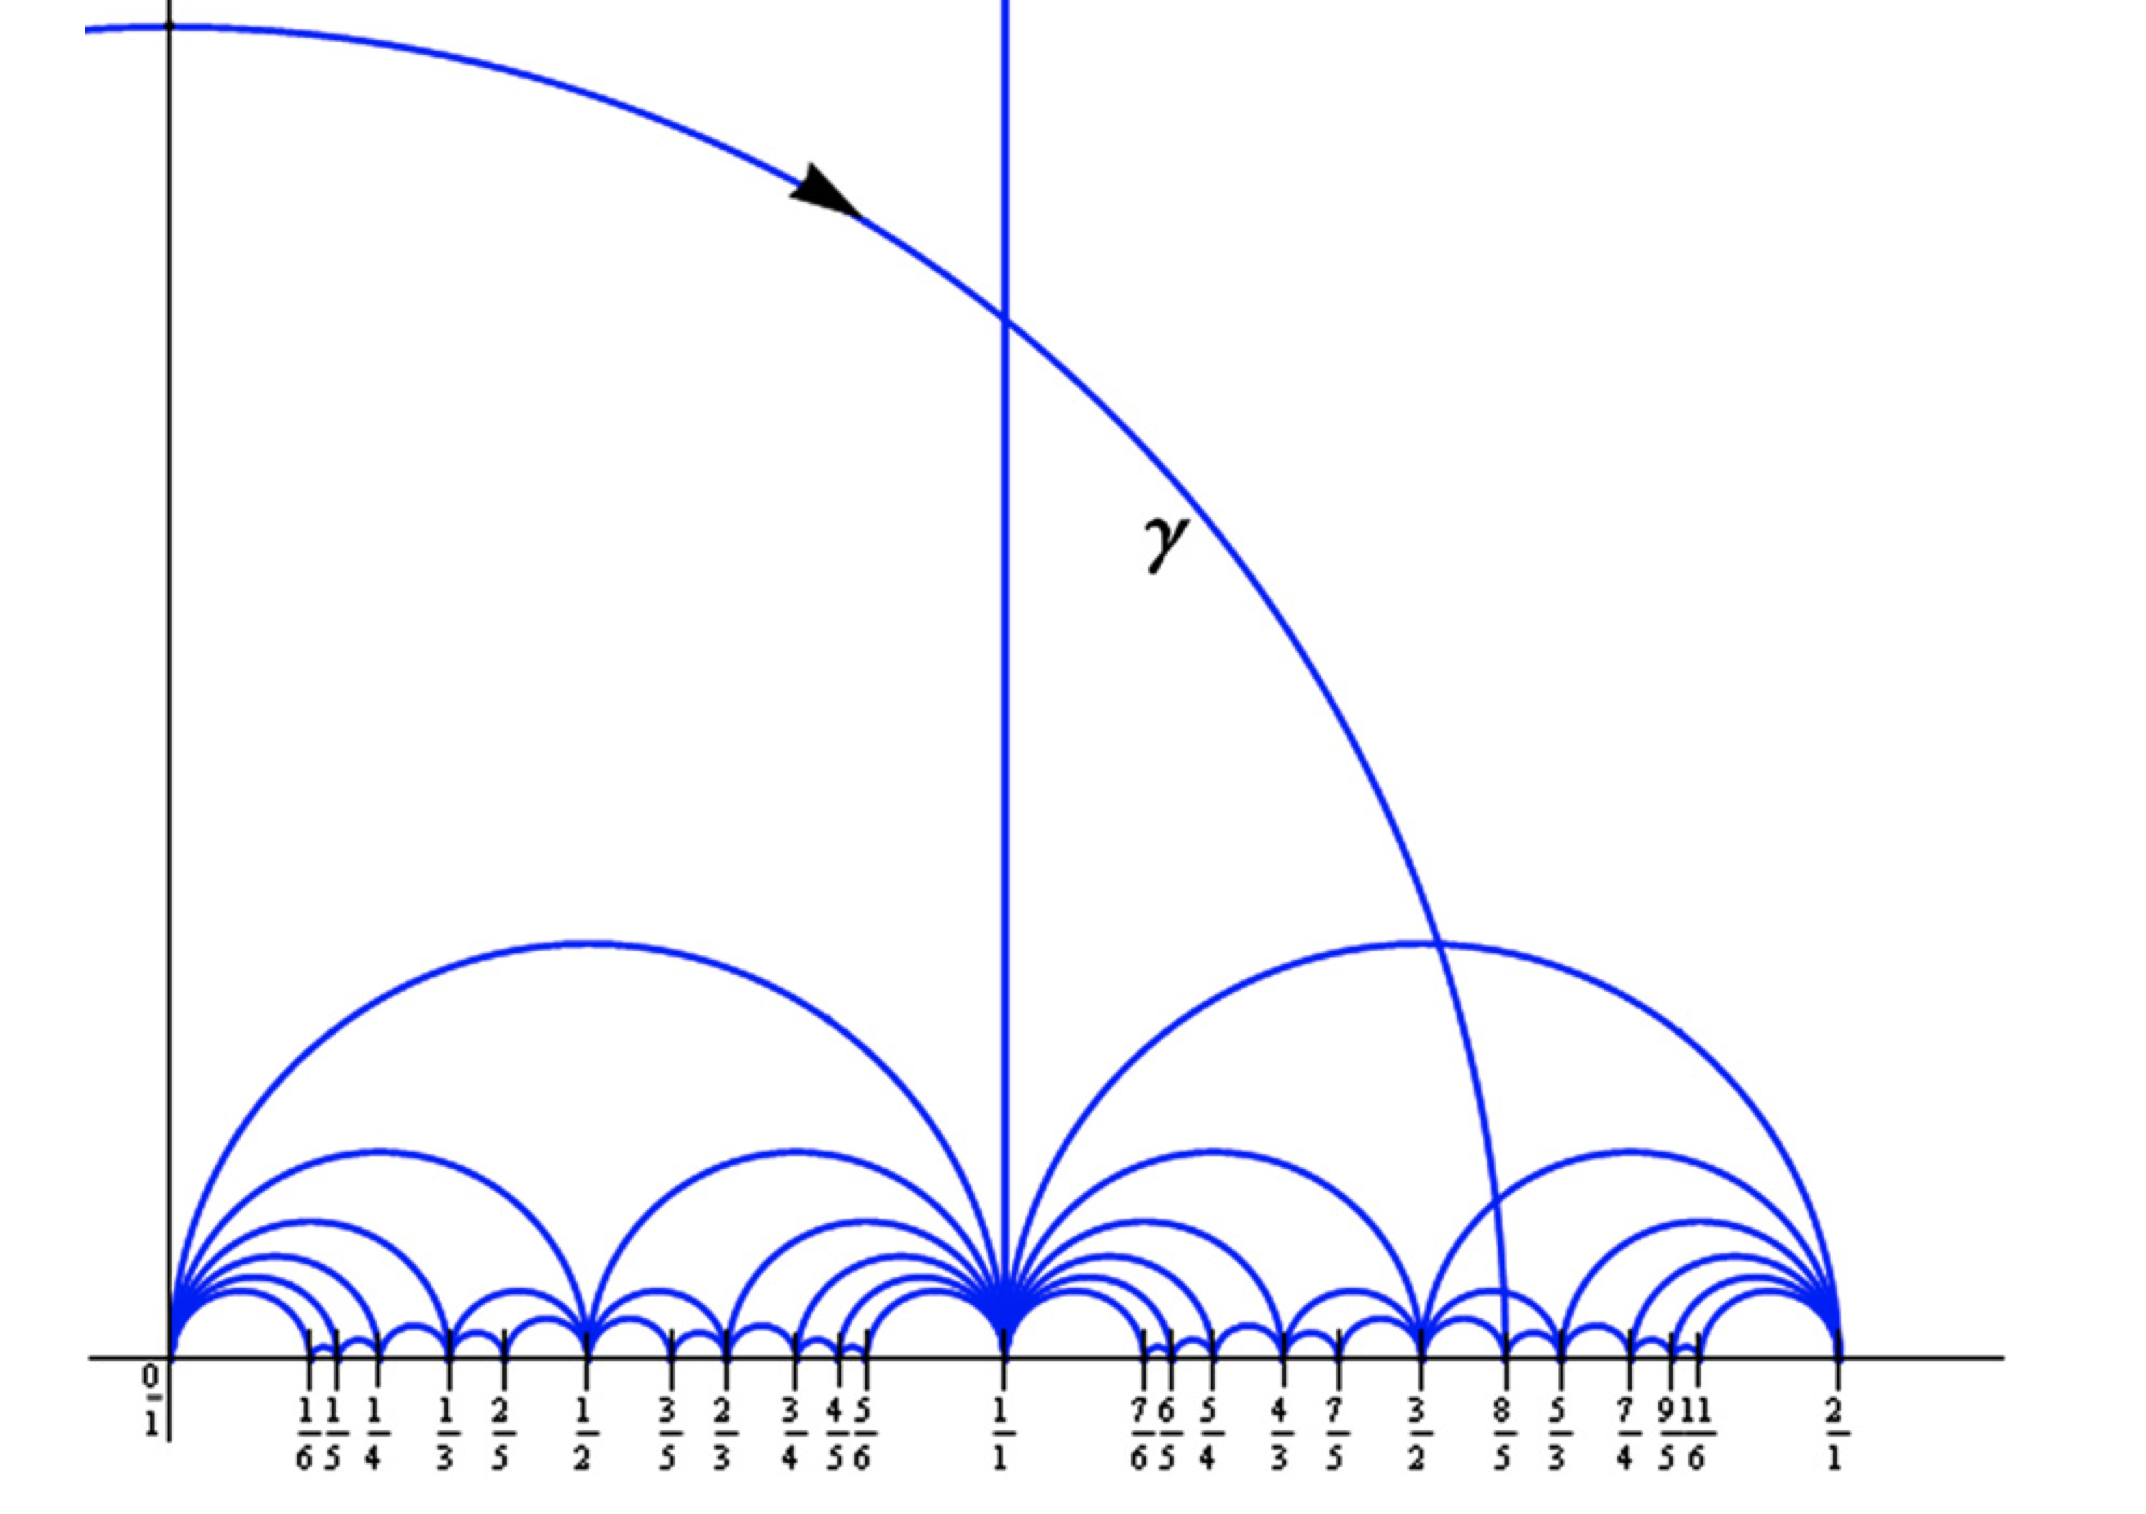
\includegraphics[scale=0.25]{pics/firstex.png}
        \caption{Exhibit A}
    \end{figure}
\end{frame}

\begin{frame}{The cutting sequence: watch and marvel}
    \begin{figure}
        \centering
        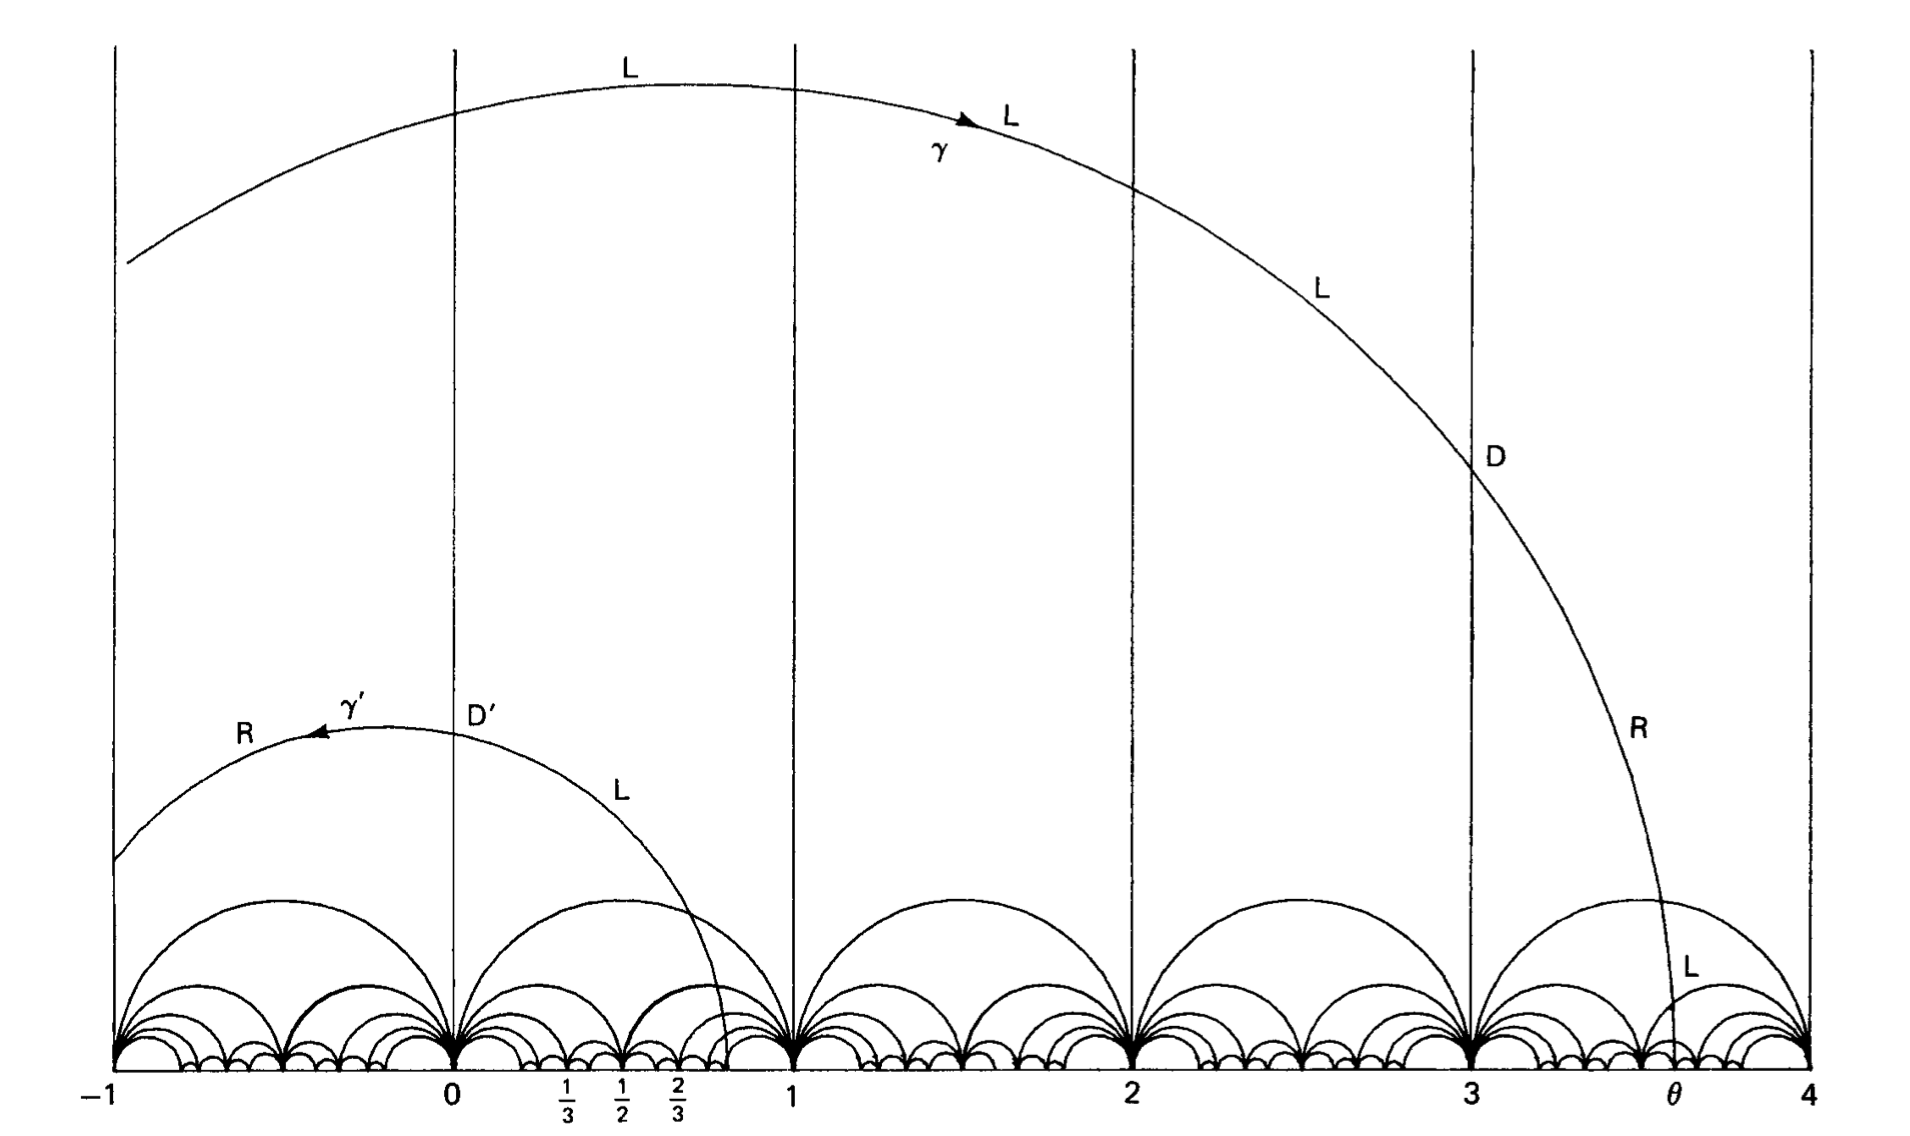
\includegraphics[scale=0.32]{pics/ex3.png}
        \caption{Exhibit B}
        \label{fig:my_label}
    \end{figure}
\end{frame}

\begin{frame}{The cutting sequence: watch and marvel}
    \begin{figure}
        \centering
        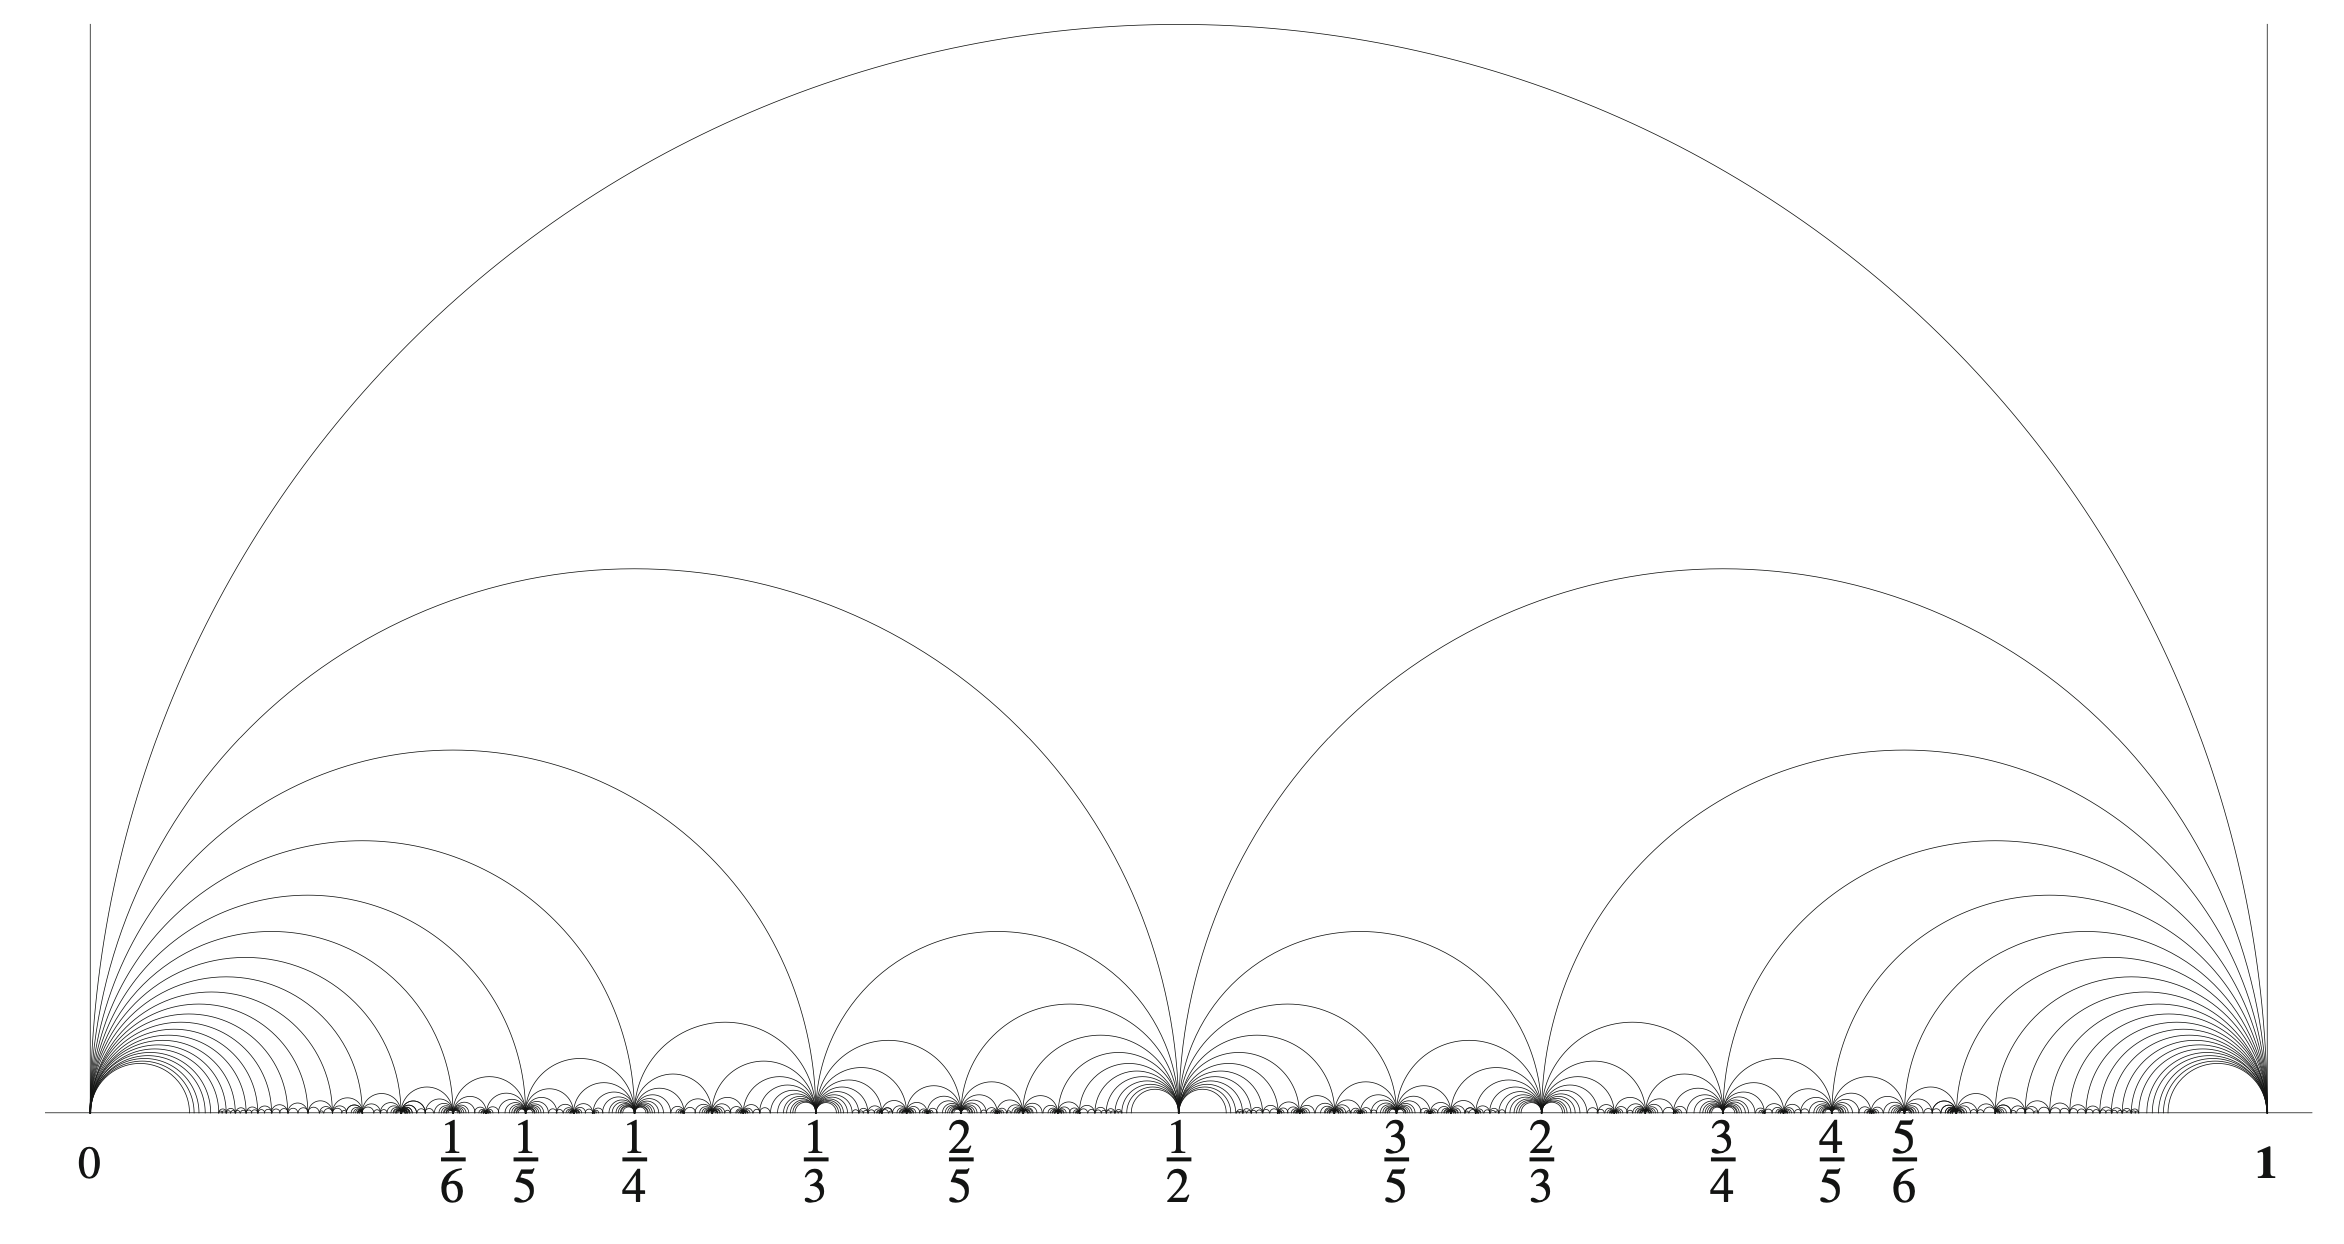
\includegraphics[scale=0.25]{pics/secondex.png}
        \caption{Exhibit C}
    \end{figure}
\end{frame}

\begin{frame}{Note}
    This is but a \emph{hint} of the astounding interplay between hyperbolic geometry and number theory. Using clever insights (in this case the Farey tessellation), a lot of geometric concepts take on special arithmetical significance! 
\end{frame}

\begin{frame}{References}
    It would be borderline criminal to be a student of number theory and never learn more about this stuff. I suggest you start with the paper which inspired this presentation:
    \begin{itemize}
        \item \emph{Continued Fractions and Hyperbolic Geometry} by Caroline Series
    \end{itemize}
    Of course, it would help to have a solid grasp of continued fractions and hyperbolic geometry, but it is by no means necessary.
\end{frame}

\end{document}
